%%
%% This is file `sample-manuscript.tex',
%% generated with the docstrip utility.
%%
%% The original source files were:
%%
%% samples.dtx  (with options: `all,proceedings,bibtex,manuscript')
%% 
%% IMPORTANT NOTICE:
%% 
%% For the copyright see the source file.
%% 
%% Any modified versions of this file must be renamed
%% with new filenames distinct from sample-manuscript.tex.
%% 
%% For distribution of the original source see the terms
%% for copying and modification in the file samples.dtx.
%% 
%% This generated file may be distributed as long as the
%% original source files, as listed above, are part of the
%% same distribution. (The sources need not necessarily be
%% in the same archive or directory.)
%%
%%
%% Commands for TeXCount
%TC:macro \cite [option:text,text]
%TC:macro \citep [option:text,text]
%TC:macro \citet [option:text,text]
%TC:envir table 0 1
%TC:envir table* 0 1
%TC:envir tabular [ignore] word
%TC:envir displaymath 0 word
%TC:envir math 0 word
%TC:envir comment 0 0
%%
%%
%% The first command in your LaTeX source must be the \documentclass
%% command.
%%
%% For submission and review of your manuscript please change the
%% command to \documentclass[manuscript, screen, review]{acmart}.
%%
%% When submitting camera ready or to TAPS, please change the command
%% to \documentclass[sigconf]{acmart} or whichever template is required
%% for your publication.
%%
%%
\documentclass[manuscript,screen,review]{acmart}
\usepackage{graphicx}
\usepackage{svg}
\usepackage{subcaption}
\usepackage{tabularx}
\usepackage{multirow}
\usepackage{standalone}
\usepackage{pgfplots}
\usepackage{csvsimple}
\usetikzlibrary{calc}
\usetikzlibrary{babel}
\usetikzlibrary{patterns}
\usepackage{geometry}
\geometry{margin=1in} 
\usepackage{pgfplotstable}
\usetikzlibrary{pgfplots.groupplots}
%%
%% \BibTeX command to typeset BibTeX logo in the docs
\AtBeginDocument{%
  \providecommand\BibTeX{{%
    Bib\TeX}}}

%% Rights management information.  This information is sent to you
%% when you complete the rights form.  These commands have SAMPLE
%% values in them; it is your responsibility as an author to replace
%% the commands and values with those provided to you when you
%% complete the rights form.
\setcopyright{acmlicensed}
\copyrightyear{2018}
\acmYear{2018}
\acmDOI{XXXXXXX.XXXXXXX}

%% These commands are for a PROCEEDINGS abstract or paper.
\acmConference[Conference acronym 'XX]{Make sure to enter the correct
  conference title from your rights confirmation emai}{June 03--05,
  2018}{Woodstock, NY}
%%
%%  Uncomment \acmBooktitle if the title of the proceedings is different
%%  from ``Proceedings of ...''!
%%
%%\acmBooktitle{Woodstock '18: ACM Symposium on Neural Gaze Detection,
%%  June 03--05, 2018, Woodstock, NY}
\acmISBN{978-1-4503-XXXX-X/18/06}


%%
%% Submission ID.
%% Use this when submitting an article to a sponsored event. You'll
%% receive a unique submission ID from the organizers
%% of the event, and this ID should be used as the parameter to this command.
%%\acmSubmissionID{123-A56-BU3}

%%
%% For managing citations, it is recommended to use bibliography
%% files in BibTeX format.
%%
%% You can then either use BibTeX with the ACM-Reference-Format style,
%% or BibLaTeX with the acmnumeric or acmauthoryear sytles, that include
%% support for advanced citation of software artefact from the
%% biblatex-software package, also separately available on CTAN.
%%
%% Look at the sample-*-biblatex.tex files for templates showcasing
%% the biblatex styles.
%%

%%
%% The majority of ACM publications use numbered citations and
%% references.  The command \citestyle{authoryear} switches to the
%% "author year" style.
%%
%% If you are preparing content for an event
%% sponsored by ACM SIGGRAPH, you must use the "author year" style of
%% citations and references.
%% Uncommenting
%% the next command will enable that style.
%%\citestyle{acmauthoryear}


%%
%% end of the preamble, start of the body of the document source.
\begin{document}

%%
%% The "title" command has an optional parameter,
%% allowing the author to define a "short title" to be used in page headers.
\title{The Name of the Title Is Hope}

%%
%% The "author" command and its associated commands are used to define
%% the authors and their affiliations.
%% Of note is the shared affiliation of the first two authors, and the
%% "authornote" and "authornotemark" commands
%% used to denote shared contribution to the research.
\author{Ben Trovato}
\authornote{Both authors contributed equally to this research.}
\email{trovato@corporation.com}
\orcid{1234-5678-9012}
\author{G.K.M. Tobin}
\authornotemark[1]
\email{webmaster@marysville-ohio.com}
\affiliation{%
  \institution{Institute for Clarity in Documentation}
  \city{Dublin}
  \state{Ohio}
  \country{USA}
}

\author{Lars Th{\o}rv{\"a}ld}
\affiliation{%
  \institution{The Th{\o}rv{\"a}ld Group}
  \city{Hekla}
  \country{Iceland}}
\email{larst@affiliation.org}

\author{Valerie B\'eranger}
\affiliation{%
  \institution{Inria Paris-Rocquencourt}
  \city{Rocquencourt}
  \country{France}
}

%%
%% By default, the full list of authors will be used in the page
%% headers. Often, this list is too long, and will overlap
%% other information printed in the page headers. This command allows
%% the author to define a more concise list
%% of authors' names for this purpose.
\renewcommand{\shortauthors}{Trovato et al.}

%%
%% The abstract is a short summary of the work to be presented in the
%% article.
\begin{abstract}
  A clear and well-documented \LaTeX\ document is presented as an
  article formatted for publication by ACM in a conference proceedings
  or journal publication. Based on the ``acmart'' document class, this
  article presents and explains many of the common variations, as well
  as many of the formatting elements an author may use in the
  preparation of the documentation of their work.
\end{abstract}

%%
%% The code below is generated by the tool at http://dl.acm.org/ccs.cfm.
%% Please copy and paste the code instead of the example below.
%%
\begin{CCSXML}
<ccs2012>
 <concept>
  <concept_id>00000000.0000000.0000000</concept_id>
  <concept_desc>Do Not Use This Code, Generate the Correct Terms for Your Paper</concept_desc>
  <concept_significance>500</concept_significance>
 </concept>
 <concept>
  <concept_id>00000000.00000000.00000000</concept_id>
  <concept_desc>Do Not Use This Code, Generate the Correct Terms for Your Paper</concept_desc>
  <concept_significance>300</concept_significance>
 </concept>
 <concept>
  <concept_id>00000000.00000000.00000000</concept_id>
  <concept_desc>Do Not Use This Code, Generate the Correct Terms for Your Paper</concept_desc>
  <concept_significance>100</concept_significance>
 </concept>
 <concept>
  <concept_id>00000000.00000000.00000000</concept_id>
  <concept_desc>Do Not Use This Code, Generate the Correct Terms for Your Paper</concept_desc>
  <concept_significance>100</concept_significance>
 </concept>
</ccs2012>
\end{CCSXML}

\ccsdesc[500]{Do Not Use This Code~Generate the Correct Terms for Your Paper}
\ccsdesc[300]{Do Not Use This Code~Generate the Correct Terms for Your Paper}
\ccsdesc{Do Not Use This Code~Generate the Correct Terms for Your Paper}
\ccsdesc[100]{Do Not Use This Code~Generate the Correct Terms for Your Paper}

%%
%% Keywords. The author(s) should pick words that accurately describe
%% the work being presented. Separate the keywords with commas.
\keywords{Do, Not, Us, This, Code, Put, the, Correct, Terms, for,
  Your, Paper}

\received{20 February 2007}
\received[revised]{12 March 2009}
\received[accepted]{5 June 2009}

%%
%% This command processes the author and affiliation and title
%% information and builds the first part of the formatted document.
\maketitle

\section{Introduction}
\section{Motivation}

% complex user code
% sparse formats and dense matrices
Several existing code matching and replacement tools rely on code structure to detect linear algebra patterns \cite{kernelfarer, IDL}. While such approaches fit well-structured naive implementations, they are prone to fail for more complex implementations. It is worth noting that that the goal of the matcher is to perform variable mapping as well as function detection. Performing such a task using a set of code patterns and constraints is extremely challenging for non-naive implementations, such as codes using AVX2 intrinsics as shown in Fig. \ref{}. Other approaches such as the ATC compiler \cite{ATC} rely on neural program classification \cite{cummins2021a} to get a set of candidate functions before examining their behavior using input/output analysis. The need for training makes extending the matcher to more function classes expensive, and makes the matching process dependent on the quality of the training data set.

Mapping the software to a hardware accelerator additionally defines some requirements for the accelerator design. First, we cannot predict the size of the input beforehand. Second, we cannot know whether the input is sparse or dense. Therefore, it is crucial that the hardware supports varying sizes, and is additionally optimized for handling dense and sparse inputs. 

Several recent works have explored SpMV acceleration on FPGA-HBM platforms \cite{hisparse, graphlily, fccm-spmv, serpens}. However, all those works are optimized for handling sparse matrices using well-known or customized sparse formats. While a dense matrix can be converted to a sparse format, such as CSR or CSC, such handling of a dense matrix would involve much unneeded overhead. First, the data required to be transferred to the accelerator is up to 3X that needed for a dense matrix. As an example, the CSR format defines three arrays: values, row pointers, and column pointers. For a sparse matrix, such a format makes sense due to the small number of non-zeros relative to the overall matrix size. For a dense matrix consisting solely of non-zeros, the three arrays invoke a large data transfer overhead. Additionally, several SpMV accelerators involve crossbars or NoCs to route matrix elements to their suitable vector banks. Such implementations cause performance overheads for dense matrices.

\subsection{Our Approach}
\subsubsection{Compiler} We design a compiler tool which relies solely on analysing a given code behaviour rather than its structure. Input/output analysis is used to determine whether the code matches a linear algebra function (GEMM or GEMV). The tool does not require training or profiling. The compiler performs variable mapping to determine variables corresponding to array sizes and constants. Next, the compiler uses the knowledge about function name and the mappings of its arguments to determine array sizes. 

\subsubsection{Profitability}
This step is crucial for determining whether offloading the function call to hardware is profitable or not. Profitability analysis is performed using a heuristic tailored for FPGA-HBM platforms, which are the target hardware. The heuristic can easily be extended to support different hardware platforms. Once the heuristic determines that execution on the FPGA-HBM is profitable, the compiler replaces the user code with a call to the accelerator.

\subsubsection{Legality} 
Behavioural equivalence methods, such as input/output testing, does not guarantee that the code is a linear algebra function. The same applies to pattern matching methods such as Kernelfarer \cite{kernelfarer}, where there is no formal proof that the code is a specific operation. However, previous work as well as our experiments \cite{ATC} have shown that, in practice, there are no false positives generated by the input/output testing method. For a more solid guarantee, a prompt can be issued to the user for confirming the detection output. 

\subsubsection{Hardware}
We design our hardware focusing on matrix-vector multiplication operations. Our accelerator supports flexible input sizes since it leverages a streaming dataflow architecture. Preprocessing is performed such that the input presented to the accelerator is optimized for both sparse and dense input matrices. Additionally, the accelerator's design ensures high performance for both input types.

\section{Related Work}

\section{Linear Algebra Code Matcher}
\subsection{Function Filtering}
We begin by loading the LLVM Intermediate Representation (IR) module of the given source file. This is achieved using llvm::LLVMContext and llvm::Module objects, which handle and store the module, respectively. The functions within the module are iterated, and metadata is employed to filter out non-user-defined functions. This ensures that our analysis focuses solely on functions defined within the provided source file, excluding those from external libraries. A heuristic is applied to identify potential GEMM and GEMV functions based on their argument types. The heuristic examines each function’s arguments to count pointers to integer, float, and double types. Functions with multiple pointer arguments and a void or pointer return are flagged as potential candidates for GEMM and GEMV.


\subsection{Input/Output Detection}
Accurate detection of input and output variables is crucial for the subsequent input/output testing step. Input-output detection involves identifying which function arguments serve as inputs (read-only) and which ones act as outputs (write-only or read-write). In other words, which arguments are livein and/or liveout variables. Liveness analysis can be performed using static analysis methods, which suits well-structured programs. However, static analysis is prone to fail for more diverse real-world codes, which may use assembly code or intrinsic functions.

Our approach uses dynamic analysis to detect which arguments are inputs and which are outputs. The function under test is executed using LLVM's Just-In-Time (JIT) compilation, with controlled input values to determine the memory behavior of each argument. In C, variables are passed by value so non-pointers variables are always livein. Our focus here is on pointer arguments (or arrays). The function is executed twice with different sets of inputs. Pointer arguments which change their value in memory are considered liveout, while the rest are livein. The second execution, with altered inputs, helps identify which variables are both livein and liveout. This dual-execution approach is critical for distinguishing between input and output arguments.

By comparing memory states before and after execution, we classify arguments as inputs, outputs, or both. Arguments with unchanged memory regions are classified as inputs, while those with changed regions are categorized as outputs. This comparison is performed by hashing the memory contents and comparing the hashes before and after function execution.

\subsection{Variable Mapping}

In the variable mapping phase, we aim to recognize which arguments of the function correspond to matrices dimensions, and which correspond to constants associated with the operation. More specifically, the GEMM and GEMV operations are represented by equations (1) and (2) respectively. The operations variables and constants are defined table \ref{variables}. Our goal is to find which, if any, of the function arguments correspond to the operation variables and constants, such that the operation matches a GEMM or a GEMV.

The General Matrix-Matrix Multiplication (GEMM) equation is given by:
\begin{equation}
	C := \alpha \cdot A \cdot B + \beta \cdot C
\end{equation}

The General Matrix-Vector Multiplication (GEMV) equation is given by:
\begin{equation}
	y := \alpha \cdot A \cdot x + \beta \cdot y
\end{equation}


\begin{table}[h!]
	\centering
	\begin{tabularx}{\textwidth}{|X|X|X|}
		\hline
		\textbf{Variable} & \textbf{GEMM} & \textbf{GEMV} \\
		\hline
		\(\alpha\) & Scalar multiplier for \(A \cdot B\) & Scalar multiplier for \(A \cdot x\) \\
		\hline
		\(\beta\) & Scalar multiplier for \(C\) & Scalar multiplier for \(y\) \\
		\hline
		\(A\) & \(m \times k\) matrix & \(m \times n\) matrix \\
		\hline
		\(B\) & \(k \times n\) matrix & \(n \times 1\) vector \\
		\hline
		\(C\) & \(m \times n\) matrix & \(m \times 1\) vector \\
		\hline
		\(lda\) & Leading dimension of \(A\) & Leading dimension of \(A\) \\
		\hline
		\(ldb\) & Leading dimension of \(B\) & Not applicable \\
		\hline
		\(ldc\) & Leading dimension of \(C\) & Not applicable \\
		\hline
	\end{tabularx}
	\caption{Comparison of variables in GEMM and GEMV}
	\label{variables}
\end{table}


The mapping algorithm we utilize is designed to dynamically verify if a given function performs matrix-matrix multiplication correctly. It leverages LLVM's JIT capabilities to execute the target function with predefined inputs and compare the outputs against expected results. The algorithm supports various data types, including float, double, and int.


The first step is defining matrix dimensions and initializing three matrices: A, B, and C. The matrices are populated with test data to serve as inputs for the target function. The mapper then analyzes the arguments of the target function to identify which arguments correspond to the matrices and their dimensions. This identification process classifies arguments into pointers (for matrices) and integers (for dimensions and constants).
The mapper iterates through possible permutations of the argument indices to determine the correct mapping of function arguments to matrices and dimensions. This exhaustive search ensures that all possible configurations are tested.

Due to the need for calling functions whose signatures are not know apriori, we utilize the foreign function interface library (libffi) to call JIT for the various permutations we test. Using the libffi library, the mapper sets up the necessary calling interface to execute the target function. The argument types and values are prepared for the JIT-compiled function call. The target function is executed with the prepared arguments. The resulting output matrix is compared against the expected result, which is computed using a reference matrix-matrix multiplication implementation. The comparison allows for a tolerance to account for floating-point inaccuracies.

\subsubsection{Classifying operations between square matrices}

As an additional verification step, we develop a recognizer model which exploits the properties of square matrices to verify the multiplication operation. Given the square matrices \(A\), \(B\), and \(C\) with order \(n\). There are no constraints on usual matrices multiplication regarding their orders. The usual matrices multiplication \(AB\) is given by Eq. \eqref{eq:mul}. We assume that the function under test performs a linear algebra operation between the matrices (multiplication, dot product, addition). Figure \ref{fig:decision-tree} shows the algorithm diagram. The multiplication operation is defined as:

\begin{equation}
	AB = \sum_{k=1}^{n} a_{ik} b_{kj}, \quad i, j = 1, \ldots, n.
	\label{eq:mul}
\end{equation}

where \(a_{ik}\) and \(b_{kj}\) are the matrix entries of \(A\) and \(B\) respectively, and \(n\) is the order of the square matrices. The multiplication property is defined as:

\begin{equation}
	 (cA)B = c(AB)
\end{equation}

For the square matrix \(A\), the trace \(\text{tr}(A)\) is defined as shown in Eq. \eqref{eq:trace}.

\begin{equation}
	\text{tr}(A) = \sum_{i=1}^{n} a_{ii}
	\label{eq:trace}
\end{equation}

The basic properties of the trace are as follows:
\begin{enumerate}
	\item \(\text{tr}(A+B) = \text{tr}(A) + \text{tr}(B)\)
	\item \(\text{tr}(\lambda A) = \lambda \text{tr}(A)\)
\end{enumerate}

where \(\lambda\) is a scalar number. Based on the multiplication and trace properties shown above, we get:

\begin{equation}
	\text{tr}(\lambda AB) = \lambda \text{tr}(AB)
	\label{eq:trace_mul}
\end{equation}

Considering that \(\text{tr}(\lambda A + B) = \lambda \text{tr}(A) + \text{tr}(B)\), we can see some differences between matrix multiplication and. for example, matrix addition with respect to the trace properties. We can use this difference to classify these matrix operations when the operators and results are known. For instance, considering the matrices \(A\), \(B\), and \(C\) such that:

\begin{equation}
	A ? B = C
	\label{eq:operation}
\end{equation}

\begin{enumerate}
	\item The square matrices \(A\), \(B\), and \(C\) must have the same order.
	\item If the operation is multiplication or dot product, the equation \(\text{tr}(\lambda AB) - \lambda \text{tr}(AB) = 0\) is true (see Eq. \eqref{eq:trace_mul}). Otherwise, the operation is addition.
	\item If \(C\) is a scalar, the operation is a dot product; otherwise, it is multiplication.
\end{enumerate}

Deriving from these properties, we first pass two random-input square matrices and check the trace property. Next, we construct the first input matrix as an upper triangular matrix. The second input matrix is filled as the identity matrix. The input data to the model consists of the following features for each test sample:
\begin{enumerate}
	\item Element \([1,n]\) of the result matrix \(C\) (last element of the first row of matrix \(C\)), denoted as \(C_{1n}\).
	\item Trace of matrix \(A\), denoted as \(\text{tr}(A)\).
	\item Element \([1,1]\) of matrix \(A\) (first element of the first row of matrix \(A\)), denoted as \(A_{11}\).
	\item Element \([1,n]\) of matrix \(B\) (last element of the first row of matrix \(B\)), denoted as \(B_{1n}\).
	\item Trace of matrix \(B\), denoted as \(\text{tr}(B)\).
	\item Trace of the result matrix \(C\), denoted as \(\text{tr}(C)\).
\end{enumerate}

The model uses these features to classify the operation performed on the matrices as follows:

\begin{itemize}
	\item \textbf{Trace Property for Addition}: The model checks if the sum of the traces of matrices \(A\) and \(B\) equals the trace of the resulting matrix \(C\):
	\[
	\text{tr}(A) + \text{tr}(B) = \text{tr}(C)
	\]
	If this condition is met (within a numerical tolerance \(\epsilon\)), the operation is classified as matrix addition.
	
	\item \textbf{Upper Triangular and Identity Matrix Property for Multiplication}: The model checks if the element \(C_{1n}\) equals the sum of the elements \(A_{11}\) and \(A_{1n}\):
	\[
	C_{1n} = A_{11} + A_{1n}
	\]
	This condition is based on the assumption that \(A\) is an upper triangular matrix and \(B\) is an identity matrix with \(B_{1n} = 1\). If this condition is met (within the numerical tolerance \(\epsilon\)), the operation is classified as matrix multiplication.
	
	\item \textbf{Other Operations}: If neither of the above conditions is met, the operation is classified as another type.
\end{itemize}

The model evaluates its performance by calculating the accuracy of its predictions compared to the true labels.



\begin{figure}[h]
	\centering
	\includesvg[scale=0.5]{svg/decision-tree.svg}
	\caption{Example SVG inclusion}
	\label{fig:decision-tree}
\end{figure}


\subsection{Size Detection}
Input size detection is an important step in our compiler toolflow, to ensure that we are offloading to the hardware only kernels which are worth offloading. In other words, the input size is required to be large enough to utilize the HBM. There are various methods in literature for input size detection. Static analysis \cite{static} is suitable for simple programs, but can fail for complex cases. Dynamic testing \cite{ATC}, by executing the function with variable sized inputs and recording points at which out-of-bound errors are reported, works well for complex codes. However, it is time consuming.

We use the knowledge about the function name and variable mappings from the previous step to locate the function call. Then, we perform a function replacement pass to replace the function with a simple function which prints the matrices dimensions and their values in the call into a csv file. Since there is no decision yet about whether it is profitable to offload the function or not, we make a copy of the original code file and perform the replacement there. After offloading profitability is analyzed, a replacement pass is performed on the original code file.

\subsection{Code Replacement}

This step is performed in the case that the offloading profitability heuristic, discussed in Section \ref{offloading-profitability}, indicates that the function should be offloaded. Since we focus in our hardware on matrix-vector multiplication, we focus here on those functions rather than the GEMM functions. The toolflow can be easily extended to support hardware accelerating GEMM. Using LLVM’s powerful code transformation capabilities, we implement a function replacement pass. This pass scans the intermediate representation (IR) of the user’s code, identifies calls to the chosen function, and replaces them with a custom function. 

The custom function, which replaces the original matrix-vector multiplication function, first converts the dense matrix to CSR format. This conversion involves extracting non-zero elements and their indices, which are then stored in a space-efficient manner. Additionally, it performs a sparsity test as this is a required input for our accelerator. The CSR matrix is saved in an NPZ file using Python’s Numpy library, which is invoked from within the C++ code via the Python C API. This NPZ file serves as input to the FPGA accelerator.

Next, we consider how to call the accelerator. Our accelerator code follows the Vitis flow. The HLS code for the accelerator is compiled as an xclbin. A C++ host program initializes the FPGA, loads the appropriate xclbin bitstream, and configures the kernels required for hardware execution. It also handles the data transfer between the host and the FPGA, executes the computation on the FPGA, and retrieves the results. The host program uses Xilinx's OpenCL runtime to interface with the FPGA. To improve modularity and ease of use, the host code is compiled as a shared library. This encapsulates the FPGA setup and execution logic, making it easier to invoke from other programs or frameworks. The library that can be dynamically linked to other applications. By compiling the host code as a library, we achieve better separation of concerns and allow for more straightforward integration with various software workflows. This library can then be linked against by the LLVM-based replacement function or other programs. The replacement function dynamically loads the shared library and calls the necessary functions to perform the matrix-vector  operation on the FPGA.



\section{Offloading Profitability Prediction}
\label{offloading-profitability}
We utilize a heuristic method we derive from our previous work, Auto-DOK \ref{autodok}, to predict the profitability of offloading a matrix-vector multiplication function to an FPGA-HBM platform. The first metric we utilize from Auto-DOK is input size. Auto-DOK identifies a threshold $(th_{in})$ at which it determines that a given input size offers good HBM PC utilization. More specifically, if the input is too small to be distributed among the HBM PCs, the bandwidth utilization degrades drastically. The access latency of HBM is not lower than that of DDR4 \cite{Shuhai,9460576}. The benefit of HBM comes from its high bandwidth. Fig. \ref{fig:example}.a. records the achieved bandwidth for a microbenchmark which performs sequential memory reads. Additionally, Fig. \ref{fig:example}.b. records the bandwidth for a matrix-vector multiplication example for different input sizes. For both benchmarks, the bandwidth is 80\% of HBM theoretical bandwidth (460 GB/s) at 64MB per PC.

The second metric is Arithmetic intensity. The Alveo U280 does not provide the FPGA with access to the host memory. Therefore, any data we need to stream must first be copied from the host to the FPGA. This data movement is expensive. We observe that for an FPGA-HBM accelerator to have a speedup over a host CPU, the kernel must exhibit enough arithmetic computations to balance the data movement cost. To quantify this, we calculate the ratio between the number of arithmetic and relational operations executed by the kernel to the size of data moved. As this definition is close to that of Arithmetic Intensity, we call this measure $AI_{cpu\rightarrow FPGA}$.

\begin{figure}%
	\centering
	\subfloat[\centering  ]{{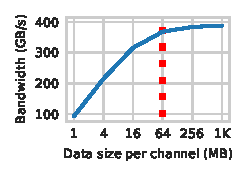
\includegraphics[width=0.4\textwidth]{pdf/seq_BW.pdf} }}%
	\qquad
	\subfloat[\centering  ]{{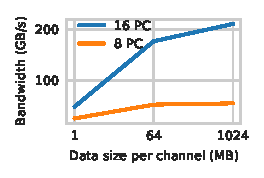
\includegraphics[width=0.4\textwidth]{pdf/mv_BW.pdf} }}%
	\caption{Bandwidth for varying input sizes. (a) Sequential memory access. (b) MV.}%
	\label{fig:example}%
\end{figure}

The thresholds, $th_{in}$ and $th_{AI}$, are tuned based on design of experiment (DoE).  
To evaluate the accuracy of the thresholds, we show the effect of varying every metric while assuming all other metrics are over their thresholds. We show results for such tests for 2 pairs of benchmarks, where each pair has similar functionality but different HLS implementations. The first pair is sparse and dense matrix-vector multiplications(MV, SpMV). The second pair are vector operation (VO), and pseudorandom access (PS). 


Fig. \ref{thresholds}.a. shows FPGA-HBM speedup over CPU when $AI_{cpu\rightarrow FPGA}$ is varied. Input per PC is set to 64MB so that it is above $th_{in}$, and the 4 benchmarks pass the regularity check. $AI_{cpu\rightarrow FPGA}$ is varied by incorporating a $Repeats$ number as explained in III.D. Similarly, Fig. \ref{thresholds}.b. shows the speedup when data size per PC is varied while keeping $AI_{cpu\rightarrow FPGA}$ above $th_{AI}$. The graphs show that at small input sizes and low arithmetic intensities, the kernels have very low (or no) speedups. Our thresholds define the metrics at which the kernels are close to achieving their maximum speedup.

\begin{figure}%
	\centering
	\subfloat[\centering  ]{{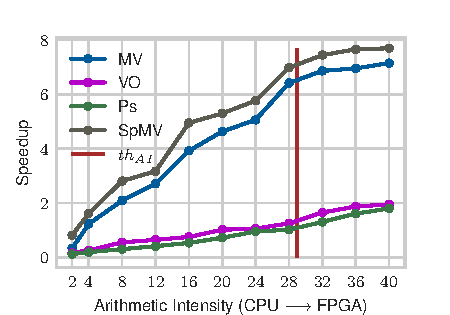
\includegraphics[width=0.4\textwidth]{pdf/AI.pdf} }}%
	\qquad
	\subfloat[\centering  ]{{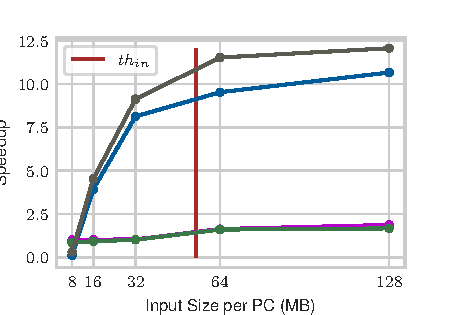
\includegraphics[width=0.4\textwidth]{pdf/in.pdf} }}%
	\caption{Effect of varying (a) $AI_{CPU\rightarrow FPGA}$. (b) $Size_{in}$ on FPGA-HBM speedup over CPU.}%
	\label{thresholds}%
\end{figure}

\section{Matrix-Vector Multiplication Acceleration on FPGA-HBM}
%fill here general overview
\subsection{Custom Matrix Format}

SpMV operation has the potential for extensive parallelism across the rows of a sparse matrix, with each row conducting a dot product with the dense vector. However, the commonly used compressed sparse row (CSR) format is not ideal for leveraging this parallelism. CSR distributes the necessary data for different processing elements (PEs) across distant memory locations, hindering both intra-channel vectorized and inter-channel concurrent memory accesses. The coordinate list format (COO) groups the element value, row, and column together, enabling random order storage of the matrix. Nonetheless, sparse matrix storage formats are not well-suited for storing dense matrices.

In this work, we propose a novel algorithm, Adaptive Cyclic Packed Streamed Rows (ACPSR), to handle sparse and dense input matrices to read the input matrix in a streamized manner without transferring unneeded information. The algorithm first partitions the matrix, then writes the matrix elements to packets whose structure varies according to the matrix type. Fig. \ref{fig:mat_format} illustrates the preprocessing steps for an architecture with 2 HBM channels.

The first step in ACPSR is partitioning the matrix along the rows and columns. Since both the vector and output are buffered on-chip, partitioning is essential to handle large matrices whose size exceeds buffer sizes. Therefore, the row partition size depends on the output buffer size, and similarly the column partition size depends on the vector buffer size.   

The next step is streamizing, which cyclically assigns rows to PEs and concatenates the rows that are assigned to one PE into one HBM channel. ACPSR marks the end of a row by inserting a special symbol (EOR) to the arrays of columns IDs and values. This approach avoids a third array for storing the row length information and simplifies the hardware design. To pack the streams assigned to a given HBM channel, ACPSR traverses the streams in a column-major order. That is, it places the first element of each stream at contiguous locations, then places the next element of of each stream at contiguous locations; this process continues until all streams run out of elements. For alignment, dummy elements are padded to the end of the shorter stream. This data placement enables all PEs to
run in parallel, each processing one stream of data.

The pack size (how many streams to pack) is adaptive depending on whether the matrix is dense or sparse. Since we can read 512 bits at a time from one HBM channel, this translates to 16 32-bit values per packet. For a sparse matrix, we need to associate column information with each element value, thereby defining the sparse pack size as 8. For a dense matrix, we already know that the column-majr traversal implies that all elements within a packet have the same column index. Therefore, we drop the column information for dense packets, leading to a dense pack size of 16. 

%explain figure? add in figure PE assignment

\begin{figure}[h]
	\centering
	\includesvg[width=\textwidth]{svg/tile-values.svg}
	\caption{Example SVG inclusion}
	\label{fig:mat_format}
\end{figure}

\subsection{Accelerator Architecture}
Fig. \ref{fig:architecture} shows an overview of the accelerator architecture. It consists of several clusters of matrix-vector computation, a vector loader, and a result draining unit. The computation clusters are memory-centric, enabling efficient streaming of both sparse and dense matrices. Additionally, the memory-centric design enables rapid scalability. Users can easily customize the hardware according to their need on various memory channels and bandwidths. All  modules are connected through streaming FIFOs in a dataflow architecture. 

The vector loader unit reads the dense vector values from HBM, and sends each cluster a copy of the data. Each computation cluster is connected to one HBM channel, where the matrix loader module reads streams of input matrix values, unpacks them to restore row indices, and distributed them to the vector read/write units. Each cluster includes four vector read/write units, which are responsible for double buffering of the incoming vector values, as well as reading out vector values according to the column index of the received matrix element. 

Eight processing elements are implemented per cluster. They perform the multiplication of the non-zero matrix element with the matching vector element, and write the result to the PE's local output buffer. The ACPSR format ensures that the row indices per packet are unique, and the hardware architecture ensures that each PE is responsible for a set of row indices in order to avoid conflicts and dependencies. After PE execution, a result packer collects all results per cluster, and sends them to the global result draining unit. This, in turn, collects cluster results and writes them back to the HBM.

%explain payloads





\begin{figure}[h]
	\centering
	\includesvg[width=\textwidth]{svg/spmv-paper.svg}
	\caption{Example SVG inclusion}
	\label{fig:architecture}
\end{figure}

\subsubsection{Matrix Loader}
The matrix loader unit is responsible for unpacking the matrix after loading from HBM by restoring its row indices, and then passing the data to the vector read/write units. Given that we use the same dataflow and the same modules for both dense and sparse input matrices,  the matrix loader unit has to adapt the size of the sparse input to match that of the dense. More specifically, the ACPSR format enables the loading 16 dense matrix elements since the column information is discarded. Therefore, the matrix loader performs zero padding after every 2 sparse elements, such that it produces 16 elements to be passed to the vector units, similar to the dense elements. Fig. \ref{fig:input-packets} illustrates the padding operation.

\begin{figure}[h]
	\centering
	\includesvg[width=\textwidth]{svg/input-packets.svg}
	\caption{Example SVG inclusion}
	\label{fig:input-packets}
\end{figure}

\subsubsection{Vector Read/Write Units}
Each PE requires random accesses to the same input dense vector. Several solutions have been proposed in recent litarature, such as crossbars and shuffle units \cite{hisparse,fccm-spmv}, in order to grant every matrix element access to the vector bank it requires. However, such solution are not a good fit for GEMV, since they introduce an extra overhead. For instance, the shuffle unit in HiSparse \cite{hisparse} implements resending logic and a crossbar to manage vector bank accesses. For input payloads with the same target output lane, the unit only grants access to one payload in a round-robin manner. Since a dense matrix packet has elements with the same column index, this causes a performance degradation, in addition to the complexity of the design which affects clock frequency.

Replicating the input vector for every PE in a separate memory is not scalable to
multiple HBM channels when using a large number of PEs. To tackle this problem, we utilize index coalescing to improve URAM utilization. More concretely, we use 4 URAMs per vector read/write unit. We refer to each URAM as a bank. The minimum bit width of a URAM configuration is 72. It is a waste to store just one vector value to one URAM address (entry). Thus, we first approximate the vector values to 18 bits, and we coalesce 4 vector values per URAM address, which we refer to as bank row. The address of a given element within a bank row is the bank column address. Thus, the vector writer and reader operate according to the following formulas:

\begin{align}
	\text{bank ID} &= \left(\frac{\text{col\_idx}}{4}\right) \% 4 \\
	\text{bank row address} &= \left(\frac{\text{col\_idx}}{16}\right) \% \text{bank\_size} \\
	\text{bank column address} &= \text{col\_idx} \% 4
\end{align}

Each cluster packs 4 vector read/write units; hence each vector unit receives 4 matrix input payloads. The URAM is configured as a two-port memory, therefore two memory reads can be performed simultaneously without violating the pipeline. In the case of sparse input, the vector unit receives two input matrix payloads and two zero paddings. Therefore, two memory accesses are performed for the first two inputs. The two resulting vector elements are written to the first two output streams. Zeros are written in the third and fourth output streams. For dense input, all input payloads have the same column index, therefore it is also sufficient to perform two memory accesses for the first 2 inputs such that the logic works for both input types. The vector values read from the two accesses are replicated for the third and fourth output streams. The vector units operations are illustrated in Fig. \ref{fig:vector-unit}.
%size of buffer?

\begin{figure}[h]
	\centering
	\includesvg[width=0.7\textwidth]{svg/vector-unit.svg}
	\caption{Example SVG inclusion}
	\label{fig:vector-unit}
\end{figure}

\subsubsection{Processing Elements with History Keeping}
The accumulation operation performed in matrix-vector multiplication over the output buffer causes read-after-write (RAW dependencies). Especially on large output buffers, such as the ones implemented in our design, the issue is demanding since both read and write consume multiple cycles, leading to more dependencies. Hence, a dynamic RAW resolution method is needed in order to fully pipeline the PE and avoid erroneous results. 

More specifically, we introduce a data structure, called the Most Recent Queue (MRQ), which acts as a shift register and keeps track of the most recent results calculated by the PE. Such a data structure enables the PE to perform load-store forwarding \cite{hisparse,graphlily} regardless of the input payload order. The MRQ stores the bank address and value per entry, and a valid bit to tackle the non-existent writes in the first cycles. Since the addition is single-stage for fixed point values, the read latency is 3, and the write latency is 2, the depth of the MRQ is chosen as 5.

% in figure we need to show PE 1 URAM
\begin{figure}[h]
	\centering
	\includesvg[width=\textwidth]{svg/pe.svg}
	\caption{Example SVG inclusion}
	\label{fig:pe}
\end{figure}

Fig. \ref{fig:pe} illustrates the overall operation of the PE. First, the PE calculates the bank address of the output buffer where the result should be written. Simultaneously, the PE performs the multiplication operation of the matrix and vector values. Next, an accumulation needs to be performed with the old (existing) value of the row. The PE checks whether the calculated bank address is found in the MRQ. If it is found, this indicates that a RAW dependency is detected. Hence, the old value is read from the MRQ. Else, it is read from the URAM. Afterwards, the MRQ is updated and the buffer write is performed. 

Similar to the vector buffer, index coalescing is used to fully utilize the URAM used for the output buffer. Each PE has its own URAM buffer, and each URAM entry consists of 4 row bank addresses. Each PE reads 2 input payloads from the vector unit. For both sparse and dense inputs, 1 read operation is required to get the old value from the output buffer. The bank address calculation is managed such that for sparse and dense inputs such that we get a fully pipelined implementation requiring only 1 write operation. The input indexes are arranged such that each PE gets 2 non-consecutive payloads. PE 0 receives payloads 0 and 2. PE 1 receives payloads 1 and 3, and so on. For the sparse input, the PE reads 1 sparse payload and a zero payload. Thus, the PE needs to perform 1 write operation for the non-zero value. For the dense input, 1 write operation is needed since we read 1 URAM word at a time, and the addresses have a difference of 2, therefore they are always within the same URAM entry.  Fig. \ref{fig:dataflow} illustrates the complete dataflow inside a cluster.


\begin{figure}[h]
	\centering
	\includesvg[width=\textwidth]{svg/dataflow.svg}
	\caption{Example SVG inclusion}
	\label{fig:pe}
\end{figure}

\subsection{Implementation Flow Enhancements}
%split kernel 
%vector loader registers
%vivado impl directives
\subsubsection{Split-Kernel Design}

Modern FPGA-HBM platforms incorporate several chip dies within a single package to
increase on-chip resources \cite{autobridge}. However, the interconnections across dies must traverse the silicon interposer, thus incurring non-trivial delays.
Moreover, in an Alveo U280 for instance, not all dies have direct connections to the HBM interface. All the HBM channels connect to a single die, Super Logic Region 0 (SLR0). A hardware module’s access to HBM would incur a long cross-die delay when the module is placed on another SLR, posing challenges to achieving timing closure.

Designing the accelerator as one monolithic kernel would pose challenges for the physical layout we described, since the floorplanner would likely be prone to crowding all the logic on the die nearer to the HBM due to the memory-centric computation clusters. This, in turn, leading to congestion and timing closure issues. Therefore, we split our design into multiple kernels, where each kernel packs several computation clusters. We set the placement of each kernel in the Vitis connectivity file, such that a balanced floorplanning is achieved among the FPGA dies. The vector loader and result draining unit are also individual kernels placed on SLR 0 to be close to the HBM.

Additionally, to broadcast vector data to all dies in the vector loader kernel, we insert extra registers and relay units to pipeline the connection, thereby avoiding costly inter-die crossings. For logic with high fan-out and high fan-in, such as vector duplication and result concatenation, we implement these as multi-level structures to enhance timing performance.


\subsubsection{CAD Directives}

AMD/Xilinx Vivado tool provides various directives to customize the FPGA implementation flow. Each directive yields different implementation outcomes. Identifying the optimal combination of directives for a specific design is challenging due to their complex behaviors and interactions. In our work, we run the tools in 'ALL' implement strategies mode, which simultaneously initiates multiple combinations of directives. We select the directive combination based on the resulting clock frequency. For Physical optimization phase, "AggressiveExplore" is chosen. For Routing, "NoTimingRelaxation" directive is selected, resulting in an clock frequency of 260MHz. All results are obtained using this combination of directives.


%\subsubsection{Design Space Exploration} 
%buffer sizes, num clusters. Alternative: mention buffer sizes in vec unit and pe subsections

\section{Compiler Evaluation}
\subsection{Experimental Setup}
The compiler tool and the native GEMM and GEMV codes are run on an AMD 1950X 2.19 GHz 16-Core machine. LLVM-14 and clang-14 were used for the compiler tool.  

\subsubsection{User Code}
For ease of comparison with state-of-the-art code detection methods, we use the same GEMM benchmarks used for evaluating the ATC compiler \cite{ATC}. These benchmarks are 50 C and C++ GEMM implementations which were collected from Github. They are categorized by the ATC compiler authors as follows: 
\begin{itemize}
	\item Naive: naive implementations with the known 3 nested loops.
	\item Naive Parallel: naive but with simple outer loop parallelization.
	\item Unrolled: naive with unrolled loops.
	\item Kernel Calls: implementations that divide the loops into different function calls.
	\item Blocked: tiled implementations.
	\item Goto: implementations of the Goto algorithm \cite{Goto}
	\item Strassen: implementations of the Strassen algorithm \cite{STRASSEN1969}
	\item Intrinsics: implementations using Intel intrinsics
\end{itemize}
In addition, we select 50 non-GEMM codes from the OJClone benchmarks and non-GEMM linear algebra code to check whether any of the approaches gave false positives. We follow the same procedure for GEMV benchmarks, where we collect user codes from Github, and select 20 programs after eliminating duplicates and programs which had compilation or implementation errors. Table \ref{gemv-codes} shows the characteristics of the test codes and their categorization.

%gemv codes

\subsubsection{Baselines}
We evaluate our approach against 5 state-of-the-art matchers:
\begin{itemize}
	\item IDL: Idioms are described using an idiom description language \cite{IDL}, which is translated into a set of constraints over LLVM IR.
	\item KernelFaRer: Uses different pattern matching to detect specific code constructs, matching specific matrix-multiplication structures \cite{kernelfarer}.
	\item FACC*: FACC uses neural embeddings and behavioral syn-
	thesis to detect candidates for acceleration \cite{facc}. FACC* improves over it by
	supporting multi-dimensional arrays.
	\item ATC: the ATC compiler uses a neural program classifier to detect regions of code that are likely to be linear algebraic operations. Afterwards, it uses input/output analysis to match user program variables with the particular API formal parameters. We share with ATC the input/output detection step which relies on monitoring argument values before and after execution, as well as the concept of using behavioral equivalence for code detection.
\end{itemize}


\subsection{Detection Accuracy}

Fig. \ref{fig:detection} shows the percentage of GEMM programs matched
by each technique across each of the 8 categories of code.
IDL was able to match only 6 cases out of 50. The reason for this is that the constraint-based matching method it uses only detects traditional implementations. The detected codes we largely in the naive category, with only 2 cases for unrolled implementations detected. Matching more complex code requires manually writing new constraints to describe each code category. KernelFaRer's patterm matching approach was more successful than IDL. It was able to detect 11 GEMMs codes. However, all the 11 detected cases were naive implementations. All other variations were undetected.

FACC*, ATC, and our approach share the broad concept of input/output testing. FACC* performed poorly on naive implementations, but better on others. the reason for this is that FACC* limits the size of the mapping search space, with a timeout of less than 10 minutes. Within this time limit, FACC* was able to 
was able to detect 10 cases. ATC is significantly more robust than the rest of the baselines across all categories, matching 42 out of 50 cases. Our approach achieves even higher accuracy than ATC, matching 45 out of the 50 cases within much less execution time. Similarly for GEMV detection, our approach achieves
90\% detection accuracy. Table \ref{gemv-codes} shows the matching result for each code.

Both our approach and ATC are able to detect all naive implementations and the majority within each other category, and are the only methods which detect GEMMs and GEMVs in codes containing kernel calls and intrinsic instructions. None of the methods classified any of the 50 non-GEMMs as a GEMM. Across all methods, there were no false positives.


%http://latexcolor.com/
\definecolor{c1}{rgb}{0.75, 0.0, 0.2}
%\definecolor{c1}{rgb}{0.8, 0.33, 0.0}
%\definecolor{c1}{rgb}{0.8, 0.33, 0.0}
%\definecolor{c1}{rgb}{1.0, 0.44, 0.37}
\definecolor{c2}{rgb}{0.0, 0.72, 0.92}
\definecolor{c4}{rgb}{0.96, 0.73, 1.0}
\definecolor{c3}{rgb}{0.98, 0.81, 0.69}
\definecolor{c5}{rgb}{0.0, 0.44, 1.0}
\definecolor{c6}{rgb}{0.0, 0.42, 0.24}

\begin{figure}[h!]
	\centering
	\includestandalone{fig-compiler-detection} % barplot.tex without the .tex extension
	\caption{Bar plot of compiler detection data.}
	\label{fig:detection}
\end{figure}


\begin{table}[h]
	\centering
	\caption{GEMV Test Cases}
	\label{tab:gemv_test_cases}
	\begin{tabular}{|l|cccc|}
		\hline
		Algorithm & Code & LoC & Optimizations & Matched? \\ \hline
		Naive & 1 & 15 & None & yes \\ \cline{2-5}
		& 2 & 26 & None & yes \\ \cline{2-5}
		& 3 & 14 & None & yes \\ \cline{2-5}
		& 4 & 30 & None & yes \\ \cline{2-5}
		& 5 & 19 & None & yes \\ \cline{2-5}
		& 6 & 22 & None & yes \\ \hline
		Parallel & 7 & 29 & OpenMP & yes \\ \cline{2-5}
		& 8 & 48 & OpenMP & yes \\ \cline{2-5}
		& 9 & 42 & OpenMP & yes \\ \cline{2-5}
		& 10 & 44 & OpenMP & yes \\ \cline{2-5}
		& 11 & 26 & C++ threads & no \\ \hline
		Unrolled & 12 & 36 & None & yes \\ \cline{2-5}
		& 13 & 34 & None & yes \\ \cline{2-5}
		& 14 & 20 & None & yes \\ \cline{2-5}
		& 15 & 76 & None & yes \\ \hline
		Vectorized & 16 & 84 & Intrinsics (AVX2) & yes \\ \cline{2-5}
		& 17 & 156 & Intrinsics (AVX2) & no \\ \cline{2-5}
		& 18 & 47 & Intrinsics (AVX2) & yes \\ \cline{2-5}
		& 19 & 35 & Intrinsics (SSE) & yes \\ \cline{2-5}
		& 20 & 188 & Intrinsics (SSE) & yes \\ \hline
	\end{tabular}
    \caption{gemv codes}
    \label{gemv-codes}
\end{table}


\subsection{Performance}

Fig. \ref{fig:execution-times} shows the total time needed to execute the tool over the 50 GEMM benchmarks. The y-axis is plotted in log scale. It can be observed from the figure that our compiler is significantly faster than ATC (45x) and FACC* (244x). There are two main reasons for being much faster than ATC. First, ATC performs input size detection by passing inputs of random sizes to the function under test, and executes it with JIT. ATC records when it receives an out-of-bounds error, and experiments until it detects the correct size. On the other hand, we perform size detection using a single replacement pass on a copy of the code, which records the input sizes in a file. The second reason is that ATC generates random inputs to test the function and records the output. This input randomness leads to the necessity of performing many experiments. For our approach , however, we rely on input and output pairs which utilize the mathematical properties of matrices. Therefore, the number experiments we require is greatly reduced.

\begin{figure}[h!]
	\centering
	\includestandalone{fig-execution-times} % barplot.tex without the .tex extension
	\caption{Bar plot of execution time (log scale).}
	\label{fig:execution-times}
\end{figure}


\section{ Hardware Evaluation and Benchmarking}

\subsection{Experimental Setup}
We implement our accelerator on AMD/Xilinx Alveo u280 using 21 HBM channels (19 for the matrix, 2 for the input and result vectors), offering a memory bandwidth of 272 GB/s. Further scaling to more than 21 HBM channels is possible, at the expense of degrading the design frequency. The accelerator is implemented in HLS using Xilinx Vitis \cite{Vitis} 2022.2.
The input vector buffer and the output vector buffer sizes are both 16 MB. We use UltraRAM (URAM), a high capacity on-chip memory, as the implementation for both buffers. The sizes of the buffers are determined by design space exploration. The pack size is 8 for sparse input and 16 for dense input, since one HBM channel delivers 512 bits per access. Our accelerator runs at runs at a frequency of 260 MHz. 

\subsubsection{CPU and GPU Baselines}

For sparse operations, we compare our accelerator with vendor-provided sparse libraries, specifically MKL (2019.5) on the CPU and cuSPARSE (10.1) on the GPU. We conduct CPU experiments using 32 threads on a two-socket 32-core 2.8 GHz Intel Xeon Gold 6242 machine with 384 GB DDR4 memory providing 282 GB/s bandwidth. GPU results are reported from \cite{hisparse}, where the experiments were run on a GTX 1080 Ti card with 3584 CUDA cores running at a peak frequency of 1582 MHz and 11 GB GDDR5X memory providing 484 GB/s bandwidth.

For dense operations, we compare against vendor-provided hipBLAS GPU library for dense linear algebra on GPUs. The results are reported from \cite{gpu-dense}, where the experiments were conducted on an AMD MI50 GPU with 16GB HBM2 memory, 60 compute units, and 3840 stream processors with peak frequency of 1 GHz.


\subsubsection{FPGA Baselines}

We are not aware of any recent work which performs matrix-vector multiplication with an optimization for both sparse and dense inputs. Therefore, we compare our accelerator with state-of-the-art FPGA sparse accelerators — HiSparse \cite{hisparse}, Serpens \cite{serpens}, FCCM23 \cite{fccm-spmv}, and Vitis Sparse Library (VSL) \cite{Xilinx2021}. All baselines target FPGAs with HBM. Similar to our design, HiSparse uses fixed-point fixed-point data types. Serpens and FCCM23 use FP32 arithmetic. VSL is an optimized HLS library released as part of the Vitis 2020.2. All baselines are open source, except for FCCm23. Additionally, the open source version of Serpens requires building with tapa \cite{tapa}. In our experiments, we encountered some version mismatch issues for building it with new releases of tapa. The released bitstream 
requires older versions of the Alveo platforms. Therefore, we use the reported results in the paper.


In our experiments, we were unable to run VSL with large matrices so we only compare with it on small datasets. We compile VSL on a Xilinx Alveo U280 platform with
16 HBM channels and 2 DDR channels providing 268 GB/s bandwidth in total. For Serpens, the authors implement a Vitis-based version and another version which uses tapa \cite{tapa} to increase frequency. We use the metrics for the Vitis-based version for fairness of comparison with the other works. 



\subsubsection{Metrics}
(1) Throughput, measured in Giga operations per second (GOPS). (2) Bandwidth efficiency, measured by throughput per unit bandwidth, in MOPS/GBPS. (3) Energy efficiency, measured by throughput per unit power, in GOPS/W.

\subsubsection{Datasets}
Table \ref{datasets} lists the matrix benchmarks used for the evaluation.
googleplus, hollywood, and pokec are social network graphs, widely used in benchmarking graph processing systems. mouse-gene is a graph from computational biology. ogbl-ppa and ogbn-products are from OGB \cite{ogb}, a benchmark suite for emerging graph neural networks. transformer-x is one layer from
a compressed Transformer \cite{transformer} model with a sparsity of x\%.


\begin{table}[h!]
	\centering
     \begin{tabular}{|l|c|c||l|c|c|}
		\hline
		\textbf{Dataset} & \textbf{Size} & \textbf{Density} & \textbf{Dataset} & \textbf{Size} & \textbf{Density} \\
		\hline
		transformer-50 & 512 × 33K & 50\% & transformer-70 & 512 × 33K & 30\% \\
		transformer-60 & 512 × 33K & 40\% & transformer-80 & 512 × 33K & 20\% \\
		transformer-90 & 512 × 33K & 10\% & transformer-95 & 512 × 33K & 5\% \\
		tsopf-rs-b2383 & 38K × 38K & 1.113 × 10\textsuperscript{-3} & mouse-gene & 45K × 45K & 1.42\% \\
		crankseg-2 & 63K × 63K & 1.75 × 10\textsuperscript{-3} & googleplus & 108K × 108K & 1.2 × 10\textsuperscript{-3} \\
		ogbl-ppa & 576K × 576K & 127.9 × 10\textsuperscript{-6} & hollywood & 1069K × 1069K & 98.5 × 10\textsuperscript{-6} \\
		pokec & 1632K × 1632K & 11.5 × 10\textsuperscript{-6} & ogbn-products & 2449K × 2449K & 20.6 × 10\textsuperscript{-6} \\
		\hline
	\end{tabular}
	\caption{Benchmark datasets with sizes and densities.}
	\label{datasets}
\end{table}

\subsection{Accelerator Evaluation}
Table \ref{cpu-gpu} shows a comparison of our accelerator with CPU and GPU baselines for sparse matrix benchmarks. Compared to MKL, our implementation has 6x higher throughput and 8.6x higher bandwidth efficiency. Compared to cuSPARSE, we achieve 1.5x higher throughput and 3.6x higher bandwidth efficiency. 

\begin{table}[h!]
	\centering
	\begin{tabular}{|l|c|c|c|c|c|c|}
		\hline
		\multirow{2}{*}{\textbf{Dataset}} & \multicolumn{3}{c|}{\textbf{Throughput (GOPS)}} & \multicolumn{3}{c|}{\textbf{Bandwidth Efficiency (MOPS/GBPS)}} \\
		\cline{2-7}
		& \textbf{MKL (CPU)} & \textbf{cuSparse (GPU)} & \textbf{Ours} & \textbf{MKL (CPU)} & \textbf{cuSparse (GPU)} & \textbf{Ours} \\
		\hline
		Transformer-50 & 5.9 & 26.9 & 34.31 & 20.9 & 55.5 & 133.87 \\		
		Transformer-60 & 5.6 & 21.5 & 31 & 19.9 & 44.5 & 129.96 \\				
		Transformer-70 & 5.2 & 17.7 & 26.48 & 18.3 & 36.6 & 131.25 \\		
		Transformer-80 & 4.1 & 19.4  & 24.54 & 14.6  & 40.1  & 118.13 \\
		Transformer-90 & 2.3 & 13.6 & 15.87 & 8.1 & 28 & 118.13 \\				
		Transformer-95 & 1.2 & 10.7 & 7.05 & 4.3 & 22.2 & 78.75 \\
		mouse-gene & 12.1 & 29 & 42.51 & 43 & 60 & 132.05 \\
		google-plus & 5.1 & 27.2 & 32.5 & 18 & 56.4 & 132.51 \\
		ogbl-ppa & 4.1 & 18 & 29.65 & 14.7 & 37.2 & 132.75 \\
		hollywood & 4.4 & 22.6 & 36.18 & 15.6 & 46.6 & 134.08 \\		
		pokec & 3 & 10.5 & 15.24 & 10.7 & 21.8 & 133.68 \\		
		ogbn-products & 3.1 & 5 & 26.8 & 11 & 10.3 & 133.98 \\						
		\hline
		
		Geometric mean & 4.06 & 16.75 & \textbf{24.5} & 14.42 & 34.62 & \textbf{124.6} \\
		\hline
	\end{tabular}
	\caption{Performance comparison between CPU (MKL), GPU (cuSparse), and our implementation, including throughput and bandwidth efficiency.}
	\label{cpu-gpu}
\end{table}

We now compare our accelerator to the accelerators dedicated for SpMV. We show the results for every baseline in a separate table to allow for a fair comparison, since not all benchmarks results are reported for all baselines.
Table \ref{vsl} shows a comparison with VSL. Our implementation is 2.2x faster than VSL, with 3.33x higher bandwidth efficiency. Regarding HiSparse, Table \ref{hisparse} shows that we outperform it by 1.5x in terms of throughput, and 1.9x in terms of bandwidth efficiency. Tables \ref{serpens} and \ref{fccm23} illustrate how our architecture compares to Serpens and FCCM23 respectively. We achieve roughly the same performance in both cases. The FCCM23 architecture was not evaluated for larger benchmarks, therefore it is not clear how to would perform for matrix sizes larger than 63K x 63K. In summary, we conclude that for sparse benchmarks, our architecture achieves the same performance as that of dedicated sparse accelerators in worst cases, and up to 2.2x higher throughput in best cases.

\begin{table}[h!]
	\centering
	\begin{tabular}{|l|c|c|c|c|}
		\hline
		\multirow{2}{*}{\textbf{Dataset}} & \multicolumn{2}{c|}{\textbf{Throughput (GOPS)}} & \multicolumn{2}{c|}{\textbf{Bandwidth Efficiency (MOPS/GBPS)}} \\
		\cline{2-5}
		& \textbf{Vitis} & \textbf{Ours} & \textbf{Vitis} & \textbf{Ours} \\
		\hline
		Transformer-50 & 17.5 & 34.31 & 65.2 & 133.87 \\
		Transformer-60 & 14.6 & 31 & 54.4 & 129.96 \\
		Transformer-70 & 13.0 & 26.48 & 48.7 & 131.25 \\
		Transformer-80 & 10.5 & 24.54 & 39.1 & 118.13 \\
		Transformer-90 & 5.8 & 15.89 & 21.8 & 118.13 \\
		Transformer-95 & 3.3 & 7.05 & 12.4 & 78.75 \\
		\hline
		Geometric mean & 9.34 & \textbf{20.64} & 34.96 & \textbf{116.57} \\
		\hline
	\end{tabular}
	\caption{Performance comparison between Vitis Sparse Library and our implementation, including throughput and bandwidth efficiency.}
	\label{vsl}
\end{table}


\begin{table}[h!]
	\centering
	\begin{tabular}{|l|c|c|c|c|}
		\hline
		\multirow{2}{*}{\textbf{Dataset}} & \multicolumn{2}{c|}{\textbf{Throughput (GOPS)}} & \multicolumn{2}{c|}{\textbf{Bandwidth Efficiency (MOPS/GBPS)}} \\
		\cline{2-5}
		& \textbf{HiSparse} & \textbf{Ours} & \textbf{HiSparse} & \textbf{Ours} \\
		\hline
		Transformer-50 & 21.9 & 34.31 & 84.7 & 133.87 \\
		Transformer-60 & 18.9 & 31 & 73.4 & 129.96 \\		
		Transformer-70 & 16.5 & 26.48 & 63.9 & 131.25 \\		
		Transformer-80 & 14.8 & 24.54 & 57.4 & 118.13 \\
		Transformer-90 & 9.7 & 15.89 & 37.8 & 118.13 \\		
		Transformer-95 & 5.7 & 7.05 & 22.0 & 78.75 \\
		mouse-gene & 27.2 & 42.52 & 105.4 & 132.05 \\
		google-plus & 21.2 & 32.5 & 82.2 & 132.51 \\
		ogbl-ppa & 24.4 & 29.65 & 94.6 & 132.75 \\
		hollywood & 24.9 & 36.18 & 96.7 & 134.08 \\
		pokec & 11.2 & 15.24 & 43.6 & 133.68 \\
		ogbn-products & 20.6 & 26.8 & 79.9 & 133.98 \\
		\hline
		Geometric mean & 16.64 & \textbf{24.5} & 64.55 & \textbf{124.6} \\
		\hline
	\end{tabular}
	\caption{Performance comparison between HiSparse and our implementation, including throughput and bandwidth efficiency.}
	\label{hisparse}
\end{table}


\begin{table}[h!]
	\centering
	\begin{minipage}{0.45\textwidth}
		\centering
		\begin{tabular}{|l|c|c|}
			\hline
			\multirow{2}{*}{\textbf{Dataset}} & \multicolumn{2}{c|}{\textbf{Throughput (GOPS)}} \\
			\cline{2-3}
			& \textbf{Serpens} & \textbf{Ours} \\
			\hline
			tsopf-rs-b2383 & 44.39 & 47.2 \\
			mouse-gene & 42.26 & 42.52 \\
			google-plus & 14.71 & 32.5 \\
			ogbl-ppa & 42.26 & 29.65 \\
			hollywood & 36.2 & 36.18 \\
			pokec & 14.29 & 15.24 \\
			ogbn-products & 39.9 & 26.8 \\
			\hline
			Geometric mean & \textbf{30.41} & \textbf{31.17} \\
			\hline
		\end{tabular}
		\caption{Performance comparison between Serpens and our implementation.}
		\label{serpens}
	\end{minipage}
	\hfill
	\begin{minipage}{0.45\textwidth}
		\centering
		\begin{tabular}{|l|c|c|}
			\hline
			\multirow{2}{*}{\textbf{Dataset}} & \multicolumn{2}{c|}{\textbf{Throughput (GOPS)}} \\
			\cline{2-3}
			& \textbf{FCCM'23} & \textbf{Ours} \\
			\hline
			mouse-gene & 38 & 42.52 \\
			tsopf-rs-b2383 & 47 & 47.2 \\
			crankseg-2 & 50.6 & 43.6491 \\
			\hline
			Geometric mean & \textbf{44.88} & \textbf{44.41} \\
			\hline
		\end{tabular}
		\caption{Performance comparison between FCCM23 and our implementation.}
		\label{fccm23}
	\end{minipage}
\end{table}

We now focus on dense benchmarks results. Matrix sizes ranging between 1024 x 1024 to 16K x 16K are tested. We attempted to obtain the performance of HiSparse with such benchmarks. However, we could only successfully run the 1024 x 1024 benchmark. Table \ref{dense} shows the throughput comparison of our architecture, HiSparse, and the hipBLAS GPU library. Our accelerator achieves 2.6x higher throughput than HiSparse. In comparison to hipBLAS, we achieve 1.26x higher throughput. The table additionally report bandwidth efficiency for our implementation, where we achieve a geometric mean of 131.17. Although we were unable to measure the dense benchmarks results for the rest of the FPGA baselines, it is very much expected that they, similar to HiSparse, achieve lower throughput than ours. The reason for this is that their dataflow is optimized for sparse benchmarks. All of the baselines can receive at most 8 matrix elements per HBM channel at a time. In contrast, we can process 16 dense elements or 8 sparse elements. Additionally, many of the baselines depend on shuffling and routing the sparse elements to their corresponding vector banks. Such optimizations fit sparse benchmarks, but degrade the performance for dense benchmarks.



\begin{table}[h!]
	\centering
	\begin{tabular}{|l|c|c|c|c|}
		\hline
		\multirow{2}{*}{\textbf{Dataset}} & \multicolumn{3}{c|}{\textbf{Throughput (GOPS)}} & \textbf{Bandwidth Efficiency (MOPS/GBPS)} \\
		\cline{2-5}
		& \textbf{HiSparse} & \textbf{hipBLAS} & \textbf{Ours} & \textbf{Ours} \\
		\hline
		1024 x 1024 & 6.99301 & 15 & 18.47 & 256 \\
		2048 x 2048 & - & 30 & 47.82 & 256 \\
		4096 x 4096 & - & 60 & 86.61 & 264 \\
		8192 x 8192 & - & 93 & 104.49 & 268 \\
		16k x 16k & - & 105 & 107.74 & 268 \\
		\hline
		Geometric mean & - & 48.33 & \textbf{61.24} & 131.17 \\
		\hline
	\end{tabular}
	\caption{Performance comparison for dense matrix-vector multiplication between HiSparse, hipBLAS, and our implementation, including throughput and bandwidth efficiency.}
	\label{dense}
\end{table}

In summary, we conclude that in terms of throughput and bandwidth efficiency, our architecture outperforms dedicated sparse accelerators, as well as several CPU and GPU libraries. In terms of FPGA resource utilization, Table \ref{resource_util} shows that the consumed resources by our architecture are comparable to the FPGA baselines, although our architecture supports optimization of both sparse and dense inputs. Finally, we examine the power and energy efficiency of the architectures. Table \ref{power_energy_efficiency}
shows the measured power consumption and energy efficiency of MKL, cuSPARSE, HiSparse, Serpens, and our implementation. Our architecture is 48x and
4.8x more energy-efficient than MKL and cuSPARSE. Additionally, our accelerator is 1.3x more energy-efficienct that HiSparse. Compared to Serpens, we achieve 76\% of its energy efficiency. 

\begin{table}[h!]
	\centering
	\begin{tabular}{|l|c|c|c|c|c|c|}
		\hline
		\textbf{Implementation} & \textbf{LUT \%} & \textbf{FF \%} & \textbf{DSP \%} & \textbf{BRAM \%} & \textbf{URAM \%} & \textbf{Frequency (MHz)} \\
		\hline
		HiSparse & 47.27 & 22.7 & 7.63 & 7.22 & 53.33 & 237 \\
		Serpens (Vitis version) & 15 & 14 & 8 & 36 & 40 & 223 \\
		FCCM23 & 38 & 45 & 7 & 23 & 40 & 310 \\
		Ours & 45 & 25.05 & 7.44 & 20.11 & 47.5 & 260 \\
		\hline
	\end{tabular}
	\caption{Resource utilization comparison among different implementations.}
	\label{resource_util}
\end{table}

\begin{table}[h!]
	\centering
	\begin{tabular}{|l|c|c|c|c|c|}
		\hline
		\textbf{} & \textbf{HiSparse} & \textbf{Serpens} & \textbf{MKL 32 threads} & \textbf{cuSPARSE} & \textbf{Ours} \\
		\hline
		\textbf{Power (W)} & 45 & 48 & 276 & 153 & 52 \\
		\textbf{Energy efficiency (GOPS/W)} & 0.37 & 0.63 & 0.01 & 0.1 & 0.48 \\
		\hline
	\end{tabular}
	\caption{Comparison of power and energy efficiency among different implementations.}
	\label{power_energy_efficiency}
\end{table}




%\section{Introduction}
%ACM's consolidated article template, introduced in 2017, provides a
%consistent \LaTeX\ style for use across ACM publications, and
%incorporates accessibility and metadata-extraction functionality
%necessary for future Digital Library endeavors. Numerous ACM and
%SIG-specific \LaTeX\ templates have been examined, and their unique
%features incorporated into this single new template.
%
%If you are new to publishing with ACM, this document is a valuable
%guide to the process of preparing your work for publication. If you
%have published with ACM before, this document provides insight and
%instruction into more recent changes to the article template.
%
%The ``\verb|acmart|'' document class can be used to prepare articles
%for any ACM publication --- conference or journal, and for any stage
%of publication, from review to final ``camera-ready'' copy, to the
%author's own version, with {\itshape very} few changes to the source.
%
%\section{Template Overview}
%As noted in the introduction, the ``\verb|acmart|'' document class can
%be used to prepare many different kinds of documentation --- a
%double-anonymous initial submission of a full-length technical paper, a
%two-page SIGGRAPH Emerging Technologies abstract, a ``camera-ready''
%journal article, a SIGCHI Extended Abstract, and more --- all by
%selecting the appropriate {\itshape template style} and {\itshape
%  template parameters}.
%
%This document will explain the major features of the document
%class. For further information, the {\itshape \LaTeX\ User's Guide} is
%available from
%\url{https://www.acm.org/publications/proceedings-template}.
%
%\subsection{Template Styles}
%
%The primary parameter given to the ``\verb|acmart|'' document class is
%the {\itshape template style} which corresponds to the kind of publication
%or SIG publishing the work. This parameter is enclosed in square
%brackets and is a part of the {\verb|documentclass|} command:
%\begin{verbatim}
%  \documentclass[STYLE]{acmart}
%\end{verbatim}
%
%Journals use one of three template styles. All but three ACM journals
%use the {\verb|acmsmall|} template style:
%\begin{itemize}
%\item {\texttt{acmsmall}}: The default journal template style.
%\item {\texttt{acmlarge}}: Used by JOCCH and TAP.
%\item {\texttt{acmtog}}: Used by TOG.
%\end{itemize}
%
%The majority of conference proceedings documentation will use the {\verb|acmconf|} template style.
%\begin{itemize}
%\item {\texttt{sigconf}}: The default proceedings template style.
%\item{\texttt{sigchi}}: Used for SIGCHI conference articles.
%\item{\texttt{sigplan}}: Used for SIGPLAN conference articles.
%\end{itemize}
%
%\subsection{Template Parameters}
%
%In addition to specifying the {\itshape template style} to be used in
%formatting your work, there are a number of {\itshape template parameters}
%which modify some part of the applied template style. A complete list
%of these parameters can be found in the {\itshape \LaTeX\ User's Guide.}
%
%Frequently-used parameters, or combinations of parameters, include:
%\begin{itemize}
%\item {\texttt{anonymous,review}}: Suitable for a ``double-anonymous''
%  conference submission. Anonymizes the work and includes line
%  numbers. Use with the \texttt{\acmSubmissionID} command to print the
%  submission's unique ID on each page of the work.
%\item{\texttt{authorversion}}: Produces a version of the work suitable
%  for posting by the author.
%\item{\texttt{screen}}: Produces colored hyperlinks.
%\end{itemize}
%
%This document uses the following string as the first command in the
%source file:
%\begin{verbatim}
%\documentclass[manuscript,screen,review]{acmart}
%\end{verbatim}
%
%\section{Modifications}
%
%Modifying the template --- including but not limited to: adjusting
%margins, typeface sizes, line spacing, paragraph and list definitions,
%and the use of the \verb|\vspace| command to manually adjust the
%vertical spacing between elements of your work --- is not allowed.
%
%{\bfseries Your document will be returned to you for revision if
%  modifications are discovered.}
%
%\section{Typefaces}
%
%The ``\verb|acmart|'' document class requires the use of the
%``Libertine'' typeface family. Your \TeX\ installation should include
%this set of packages. Please do not substitute other typefaces. The
%``\verb|lmodern|'' and ``\verb|ltimes|'' packages should not be used,
%as they will override the built-in typeface families.
%
%\section{Title Information}
%
%The title of your work should use capital letters appropriately -
%\url{https://capitalizemytitle.com/} has useful rules for
%capitalization. Use the {\verb|title|} command to define the title of
%your work. If your work has a subtitle, define it with the
%{\verb|subtitle|} command.  Do not insert line breaks in your title.
%
%If your title is lengthy, you must define a short version to be used
%in the page headers, to prevent overlapping text. The \verb|title|
%command has a ``short title'' parameter:
%\begin{verbatim}
%  \title[short title]{full title}
%\end{verbatim}
%
%\section{Authors and Affiliations}
%
%Each author must be defined separately for accurate metadata
%identification.  As an exception, multiple authors may share one
%affiliation. Authors' names should not be abbreviated; use full first
%names wherever possible. Include authors' e-mail addresses whenever
%possible.
%
%Grouping authors' names or e-mail addresses, or providing an ``e-mail
%alias,'' as shown below, is not acceptable:
%\begin{verbatim}
%  \author{Brooke Aster, David Mehldau}
%  \email{dave,judy,steve@university.edu}
%  \email{firstname.lastname@phillips.org}
%\end{verbatim}
%
%The \verb|authornote| and \verb|authornotemark| commands allow a note
%to apply to multiple authors --- for example, if the first two authors
%of an article contributed equally to the work.
%
%If your author list is lengthy, you must define a shortened version of
%the list of authors to be used in the page headers, to prevent
%overlapping text. The following command should be placed just after
%the last \verb|\author{}| definition:
%\begin{verbatim}
%  \renewcommand{\shortauthors}{McCartney, et al.}
%\end{verbatim}
%Omitting this command will force the use of a concatenated list of all
%of the authors' names, which may result in overlapping text in the
%page headers.
%
%The article template's documentation, available at
%\url{https://www.acm.org/publications/proceedings-template}, has a
%complete explanation of these commands and tips for their effective
%use.
%
%Note that authors' addresses are mandatory for journal articles.
%
%\section{Rights Information}
%
%Authors of any work published by ACM will need to complete a rights
%form. Depending on the kind of work, and the rights management choice
%made by the author, this may be copyright transfer, permission,
%license, or an OA (open access) agreement.
%
%Regardless of the rights management choice, the author will receive a
%copy of the completed rights form once it has been submitted. This
%form contains \LaTeX\ commands that must be copied into the source
%document. When the document source is compiled, these commands and
%their parameters add formatted text to several areas of the final
%document:
%\begin{itemize}
%\item the ``ACM Reference Format'' text on the first page.
%\item the ``rights management'' text on the first page.
%\item the conference information in the page header(s).
%\end{itemize}
%
%Rights information is unique to the work; if you are preparing several
%works for an event, make sure to use the correct set of commands with
%each of the works.
%
%The ACM Reference Format text is required for all articles over one
%page in length, and is optional for one-page articles (abstracts).
%
%\section{CCS Concepts and User-Defined Keywords}
%
%Two elements of the ``acmart'' document class provide powerful
%taxonomic tools for you to help readers find your work in an online
%search.
%
%The ACM Computing Classification System ---
%\url{https://www.acm.org/publications/class-2012} --- is a set of
%classifiers and concepts that describe the computing
%discipline. Authors can select entries from this classification
%system, via \url{https://dl.acm.org/ccs/ccs.cfm}, and generate the
%commands to be included in the \LaTeX\ source.
%
%User-defined keywords are a comma-separated list of words and phrases
%of the authors' choosing, providing a more flexible way of describing
%the research being presented.
%
%CCS concepts and user-defined keywords are required for for all
%articles over two pages in length, and are optional for one- and
%two-page articles (or abstracts).
%
%\section{Sectioning Commands}
%
%Your work should use standard \LaTeX\ sectioning commands:
%\verb|section|, \verb|subsection|, \verb|subsubsection|, and
%\verb|paragraph|. They should be numbered; do not remove the numbering
%from the commands.
%
%Simulating a sectioning command by setting the first word or words of
%a paragraph in boldface or italicized text is {\bfseries not allowed.}
%
%\section{Tables}
%
%The ``\verb|acmart|'' document class includes the ``\verb|booktabs|''
%package --- \url{https://ctan.org/pkg/booktabs} --- for preparing
%high-quality tables.
%
%Table captions are placed {\itshape above} the table.
%
%Because tables cannot be split across pages, the best placement for
%them is typically the top of the page nearest their initial cite.  To
%ensure this proper ``floating'' placement of tables, use the
%environment \textbf{table} to enclose the table's contents and the
%table caption.  The contents of the table itself must go in the
%\textbf{tabular} environment, to be aligned properly in rows and
%columns, with the desired horizontal and vertical rules.  Again,
%detailed instructions on \textbf{tabular} material are found in the
%\textit{\LaTeX\ User's Guide}.
%
%Immediately following this sentence is the point at which
%Table~\ref{tab:freq} is included in the input file; compare the
%placement of the table here with the table in the printed output of
%this document.
%
%\begin{table}
%  \caption{Frequency of Special Characters}
%  \label{tab:freq}
%  \begin{tabular}{ccl}
%    \toprule
%    Non-English or Math&Frequency&Comments\\
%    \midrule
%    \O & 1 in 1,000& For Swedish names\\
%    $\pi$ & 1 in 5& Common in math\\
%    \$ & 4 in 5 & Used in business\\
%    $\Psi^2_1$ & 1 in 40,000& Unexplained usage\\
%  \bottomrule
%\end{tabular}
%\end{table}
%
%To set a wider table, which takes up the whole width of the page's
%live area, use the environment \textbf{table*} to enclose the table's
%contents and the table caption.  As with a single-column table, this
%wide table will ``float'' to a location deemed more
%desirable. Immediately following this sentence is the point at which
%Table~\ref{tab:commands} is included in the input file; again, it is
%instructive to compare the placement of the table here with the table
%in the printed output of this document.
%
%\begin{table*}
%  \caption{Some Typical Commands}
%  \label{tab:commands}
%  \begin{tabular}{ccl}
%    \toprule
%    Command &A Number & Comments\\
%    \midrule
%    \texttt{{\char'134}author} & 100& Author \\
%    \texttt{{\char'134}table}& 300 & For tables\\
%    \texttt{{\char'134}table*}& 400& For wider tables\\
%    \bottomrule
%  \end{tabular}
%\end{table*}
%
%Always use midrule to separate table header rows from data rows, and
%use it only for this purpose. This enables assistive technologies to
%recognise table headers and support their users in navigating tables
%more easily.
%
%\section{Math Equations}
%You may want to display math equations in three distinct styles:
%inline, numbered or non-numbered display.  Each of the three are
%discussed in the next sections.
%
%\subsection{Inline (In-text) Equations}
%A formula that appears in the running text is called an inline or
%in-text formula.  It is produced by the \textbf{math} environment,
%which can be invoked with the usual
%\texttt{{\char'134}begin\,\ldots{\char'134}end} construction or with
%the short form \texttt{\$\,\ldots\$}. You can use any of the symbols
%and structures, from $\alpha$ to $\omega$, available in
%\LaTeX~\cite{Lamport:LaTeX}; this section will simply show a few
%examples of in-text equations in context. Notice how this equation:
%\begin{math}
%  \lim_{n\rightarrow \infty}x=0
%\end{math},
%set here in in-line math style, looks slightly different when
%set in display style.  (See next section).
%
%\subsection{Display Equations}
%A numbered display equation---one set off by vertical space from the
%text and centered horizontally---is produced by the \textbf{equation}
%environment. An unnumbered display equation is produced by the
%\textbf{displaymath} environment.
%
%Again, in either environment, you can use any of the symbols and
%structures available in \LaTeX\@; this section will just give a couple
%of examples of display equations in context.  First, consider the
%equation, shown as an inline equation above:
%\begin{equation}
%  \lim_{n\rightarrow \infty}x=0
%\end{equation}
%Notice how it is formatted somewhat differently in
%the \textbf{displaymath}
%environment.  Now, we'll enter an unnumbered equation:
%\begin{displaymath}
%  \sum_{i=0}^{\infty} x + 1
%\end{displaymath}
%and follow it with another numbered equation:
%\begin{equation}
%  \sum_{i=0}^{\infty}x_i=\int_{0}^{\pi+2} f
%\end{equation}
%just to demonstrate \LaTeX's able handling of numbering.
%
%\section{Figures}
%
%The ``\verb|figure|'' environment should be used for figures. One or
%more images can be placed within a figure. If your figure contains
%third-party material, you must clearly identify it as such, as shown
%in the example below.
%\begin{figure}[h]
%  \centering
%  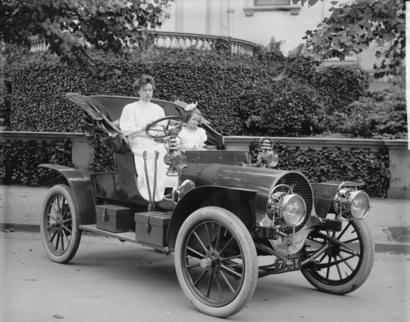
\includegraphics[width=\linewidth]{sample-franklin}
%  \caption{1907 Franklin Model D roadster. Photograph by Harris \&
%    Ewing, Inc. [Public domain], via Wikimedia
%    Commons. (\url{https://goo.gl/VLCRBB}).}
%  \Description{A woman and a girl in white dresses sit in an open car.}
%\end{figure}
%
%Your figures should contain a caption which describes the figure to
%the reader.
%
%Figure captions are placed {\itshape below} the figure.
%
%Every figure should also have a figure description unless it is purely
%decorative. These descriptions convey what’s in the image to someone
%who cannot see it. They are also used by search engine crawlers for
%indexing images, and when images cannot be loaded.
%
%A figure description must be unformatted plain text less than 2000
%characters long (including spaces).  {\bfseries Figure descriptions
%  should not repeat the figure caption – their purpose is to capture
%  important information that is not already provided in the caption or
%  the main text of the paper.} For figures that convey important and
%complex new information, a short text description may not be
%adequate. More complex alternative descriptions can be placed in an
%appendix and referenced in a short figure description. For example,
%provide a data table capturing the information in a bar chart, or a
%structured list representing a graph.  For additional information
%regarding how best to write figure descriptions and why doing this is
%so important, please see
%\url{https://www.acm.org/publications/taps/describing-figures/}.
%
%\subsection{The ``Teaser Figure''}
%
%A ``teaser figure'' is an image, or set of images in one figure, that
%are placed after all author and affiliation information, and before
%the body of the article, spanning the page. If you wish to have such a
%figure in your article, place the command immediately before the
%\verb|\maketitle| command:
%\begin{verbatim}
%  \begin{teaserfigure}
%    \includegraphics[width=\textwidth]{sampleteaser}
%    \caption{figure caption}
%    \Description{figure description}
%  \end{teaserfigure}
%\end{verbatim}
%
%\section{Citations and Bibliographies}
%
%The use of \BibTeX\ for the preparation and formatting of one's
%references is strongly recommended. Authors' names should be complete
%--- use full first names (``Donald E. Knuth'') not initials
%(``D. E. Knuth'') --- and the salient identifying features of a
%reference should be included: title, year, volume, number, pages,
%article DOI, etc.
%
%The bibliography is included in your source document with these two
%commands, placed just before the \verb|\end{document}| command:
%\begin{verbatim}
%  \bibliographystyle{ACM-Reference-Format}
%  \bibliography{bibfile}
%\end{verbatim}
%where ``\verb|bibfile|'' is the name, without the ``\verb|.bib|''
%suffix, of the \BibTeX\ file.
%
%Citations and references are numbered by default. A small number of
%ACM publications have citations and references formatted in the
%``author year'' style; for these exceptions, please include this
%command in the {\bfseries preamble} (before the command
%``\verb|\begin{document}|'') of your \LaTeX\ source:
%\begin{verbatim}
%  \citestyle{acmauthoryear}
%\end{verbatim}
%
%
%  Some examples.  A paginated journal article \cite{Abril07}, an
%  enumerated journal article \cite{Cohen07}, a reference to an entire
%  issue \cite{JCohen96}, a monograph (whole book) \cite{Kosiur01}, a
%  monograph/whole book in a series (see 2a in spec. document)
%  \cite{Harel79}, a divisible-book such as an anthology or compilation
%  \cite{Editor00} followed by the same example, however we only output
%  the series if the volume number is given \cite{Editor00a} (so
%  Editor00a's series should NOT be present since it has no vol. no.),
%  a chapter in a divisible book \cite{Spector90}, a chapter in a
%  divisible book in a series \cite{Douglass98}, a multi-volume work as
%  book \cite{Knuth97}, a couple of articles in a proceedings (of a
%  conference, symposium, workshop for example) (paginated proceedings
%  article) \cite{Andler79, Hagerup1993}, a proceedings article with
%  all possible elements \cite{Smith10}, an example of an enumerated
%  proceedings article \cite{VanGundy07}, an informally published work
%  \cite{Harel78}, a couple of preprints \cite{Bornmann2019,
%    AnzarootPBM14}, a doctoral dissertation \cite{Clarkson85}, a
%  master's thesis: \cite{anisi03}, an online document / world wide web
%  resource \cite{Thornburg01, Ablamowicz07, Poker06}, a video game
%  (Case 1) \cite{Obama08} and (Case 2) \cite{Novak03} and \cite{Lee05}
%  and (Case 3) a patent \cite{JoeScientist001}, work accepted for
%  publication \cite{rous08}, 'YYYYb'-test for prolific author
%  \cite{SaeediMEJ10} and \cite{SaeediJETC10}. Other cites might
%  contain 'duplicate' DOI and URLs (some SIAM articles)
%  \cite{Kirschmer:2010:AEI:1958016.1958018}. Boris / Barbara Beeton:
%  multi-volume works as books \cite{MR781536} and \cite{MR781537}. A
%  couple of citations with DOIs:
%  \cite{2004:ITE:1009386.1010128,Kirschmer:2010:AEI:1958016.1958018}. Online
%  citations: \cite{TUGInstmem, Thornburg01, CTANacmart}.
%  Artifacts: \cite{R} and \cite{UMassCitations}.
%
%\section{Acknowledgments}
%
%Identification of funding sources and other support, and thanks to
%individuals and groups that assisted in the research and the
%preparation of the work should be included in an acknowledgment
%section, which is placed just before the reference section in your
%document.
%
%This section has a special environment:
%\begin{verbatim}
%  \begin{acks}
%  ...
%  \end{acks}
%\end{verbatim}
%so that the information contained therein can be more easily collected
%during the article metadata extraction phase, and to ensure
%consistency in the spelling of the section heading.
%
%Authors should not prepare this section as a numbered or unnumbered {\verb|\section|}; please use the ``{\verb|acks|}'' environment.
%
%\section{Appendices}
%
%If your work needs an appendix, add it before the
%``\verb|\end{document}|'' command at the conclusion of your source
%document.
%
%Start the appendix with the ``\verb|appendix|'' command:
%\begin{verbatim}
%  \appendix
%\end{verbatim}
%and note that in the appendix, sections are lettered, not
%numbered. This document has two appendices, demonstrating the section
%and subsection identification method.
%
%\section{Multi-language papers}
%
%Papers may be written in languages other than English or include
%titles, subtitles, keywords and abstracts in different languages (as a
%rule, a paper in a language other than English should include an
%English title and an English abstract).  Use \verb|language=...| for
%every language used in the paper.  The last language indicated is the
%main language of the paper.  For example, a French paper with
%additional titles and abstracts in English and German may start with
%the following command
%\begin{verbatim}
%\documentclass[sigconf, language=english, language=german,
%               language=french]{acmart}
%\end{verbatim}
%
%The title, subtitle, keywords and abstract will be typeset in the main
%language of the paper.  The commands \verb|\translatedXXX|, \verb|XXX|
%begin title, subtitle and keywords, can be used to set these elements
%in the other languages.  The environment \verb|translatedabstract| is
%used to set the translation of the abstract.  These commands and
%environment have a mandatory first argument: the language of the
%second argument.  See \verb|sample-sigconf-i13n.tex| file for examples
%of their usage.
%
%\section{SIGCHI Extended Abstracts}
%
%The ``\verb|sigchi-a|'' template style (available only in \LaTeX\ and
%not in Word) produces a landscape-orientation formatted article, with
%a wide left margin. Three environments are available for use with the
%``\verb|sigchi-a|'' template style, and produce formatted output in
%the margin:
%\begin{description}
%\item[\texttt{sidebar}:]  Place formatted text in the margin.
%\item[\texttt{marginfigure}:] Place a figure in the margin.
%\item[\texttt{margintable}:] Place a table in the margin.
%\end{description}
%
%%%
%%% The acknowledgments section is defined using the "acks" environment
%%% (and NOT an unnumbered section). This ensures the proper
%%% identification of the section in the article metadata, and the
%%% consistent spelling of the heading.
%\begin{acks}
%To Robert, for the bagels and explaining CMYK and color spaces.
%\end{acks}
%
%%%
%%% The next two lines define the bibliography style to be used, and
%%% the bibliography file.
%\bibliographystyle{ACM-Reference-Format}
%\bibliography{sample-base}
%
%
%%%
%%% If your work has an appendix, this is the place to put it.
%\appendix
%
%\section{Research Methods}
%
%\subsection{Part One}
%
%Lorem ipsum dolor sit amet, consectetur adipiscing elit. Morbi
%malesuada, quam in pulvinar varius, metus nunc fermentum urna, id
%sollicitudin purus odio sit amet enim. Aliquam ullamcorper eu ipsum
%vel mollis. Curabitur quis dictum nisl. Phasellus vel semper risus, et
%lacinia dolor. Integer ultricies commodo sem nec semper.
%
%\subsection{Part Two}
%
%Etiam commodo feugiat nisl pulvinar pellentesque. Etiam auctor sodales
%ligula, non varius nibh pulvinar semper. Suspendisse nec lectus non
%ipsum convallis congue hendrerit vitae sapien. Donec at laoreet
%eros. Vivamus non purus placerat, scelerisque diam eu, cursus
%ante. Etiam aliquam tortor auctor efficitur mattis.
%
%\section{Online Resources}
%
%Nam id fermentum dui. Suspendisse sagittis tortor a nulla mollis, in
%pulvinar ex pretium. Sed interdum orci quis metus euismod, et sagittis
%enim maximus. Vestibulum gravida massa ut felis suscipit
%congue. Quisque mattis elit a risus ultrices commodo venenatis eget
%dui. Etiam sagittis eleifend elementum.
%
%Nam interdum magna at lectus dignissim, ac dignissim lorem
%rhoncus. Maecenas eu arcu ac neque placerat aliquam. Nunc pulvinar
%massa et mattis lacinia.
\bibliographystyle{ACM-Reference-Format}
\bibliography{references.bib}
\end{document}
\endinput
%%
%% End of file `sample-manuscript.tex'.
